\frame{\titlepage}

\section{Знаковая природа языка и антиномии языковой системы}

\frame{\tableofcontents[currentsection]}

\begin{frame}{Язык как система знаков}
    \begin{block}{Система}
        Множество элементов, находящихся в отношениях и связях друг с другом, которое образует определённую целостность, единство.
    \end{block}

    \begin{block}{Знак}
        Материально-идеальное образование, обозначающее предмет, свойство, отношение действительности.
    \end{block}

    \vfill

    \begin{alertblock}{Закон знака (В.~фон Гумбольдт)}
        Универсальный принцип строения языков~"--- единство значения \textbf{(означаемого)} и формы его выражения \textbf{(означающего)}.
    \end{alertblock}
\end{frame}

\begin{frame}{Семиотические триады}
    \begin{block}{Ч.~Пирс}
        Три типа знаков по характеру связи между означаемым и означающим: \begin{itemize}
            \item иконические: метафора
            \item индексы: метонимия
            \item символы: связь чисто условная
        \end{itemize}
    \end{block}

    \begin{block}{Ч.~Моррис}
        Три семиотические сферы: \begin{itemize}
            \item семантика: отношение знака к объекту (денотату)
            \item \alert{синтактика}: отношение знаков между собой
            \item прагматика: отношение знака к субъекту
        \end{itemize}
    \end{block}
\end{frame}

\begin{frame}{Глоссематика}
    \begin{table}[t]
        \begin{tabularx}{\textwidth}{XXXX}
            \multicolumn{2}{c}{План выражения} & \multicolumn{2}{c}{План содержания} \\ \midrule
            Субстанция & Форма & Форма & Субстанция \\ \midrule
            & Кенематика & Плерематика & \\ \midrule
            Фонетика & \multicolumn{2}{c}{Глоссематика} & Семантика \\
        \end{tabularx}
    \end{table}
\end{frame}

\begin{frame}{Соссюровские антиномии}
    \begin{columns}
        \column{.5\textwidth}
        \begin{itemize}
            \item Язык
            \item Синхрония
            \item Ассоциативные отношения
            \item Внутренняя лингвистика
        \end{itemize}

        \column{.5\textwidth}
        \begin{itemize}
            \item Речь
            \item Диахрония
            \item Синтагматические отношения
            \item Внешняя лингвистика
        \end{itemize}
    \end{columns}
\end{frame}

\begin{frame}{Язык, речь, языковая деятельность}
    \begin{columns}
        \column{.5\textwidth}
        \begin{block}{Язык (la langue)}
            Система единиц и правил для создания речевых произведений
            \begin{itemize}
                \item Социален
                \item Потенциален
                \item Психичен
            \end{itemize}
        \end{block}

        \column{.5\textwidth}
        \begin{block}{Речь (la parole)}
            Активное использование языка в соответствии с мыслью говорящего
            \begin{itemize}
                \item Индивидуальна
                \item Актуальна
                \item Материальна
            \end{itemize}
        \end{block}
    \end{columns}

    \vfill

    \begin{block}{Языковая деятельность (le langage)}
        Речь $+$ экстралингвистические факторы
    \end{block}
\end{frame}

\begin{frame}{Трихотомия Щербы}
    \begin{block}{Речевая деятельность}
        Совокупность всего говоримого и слышимого отдельным индивидом
    \end{block}

    \begin{block}{Языковой материал}
        То же, но на синхронном срезе
    \end{block}

    \begin{block}{Языковая система}
        $\sim$ Язык у Соссюра
    \end{block}
\end{frame}

\begin{frame}{Текст и дискурс}
    \begin{quote}
        Язык выше уровня предложения (З.~Харрис)
    \end{quote}

    \begin{columns}
        \column{.5\textwidth}
        \begin{block}{Текст}
            \begin{itemize}
                \item Дискурс $-$ ситуация
                \item Теор.\ конструкт (ср.\ предложение)
                \item Продукт
            \end{itemize}
        \end{block}

        \column{.5\textwidth}
        \begin{block}{Дискурс}
            \begin{itemize}
                \item Текст $+$ ситуация
                \item Актуализация (ср.\ высказывание)
                \item Процесс
            \end{itemize}
        \end{block}
    \end{columns}
\end{frame}

\begin{frame}{Парадигматика и синтагматика}
    \begin{quote}
        Парадигматика $\sim$ \textit{вместо}, синтагматика $\sim$ \textit{вместе} (И.\,А.~Мельчук)
    \end{quote}
\end{frame}

\begin{frame}{Классификация языков между собой}
    \begin{table}[t]
        \begin{tabularx}{\textwidth}{p{3cm}XXX}
            & Генеалогическая & Типологическая & Ареальная \\ \midrule \midrule
            Ключевое понятие & Родство & Строй & Ареал \\ \midrule
            Русский язык
                & Индоевропейская семья \linebreak \mbox{Славянская} ветвь \linebreak Восточнославянская группа
                & Фонемный \linebreak Флективный \linebreak SVO
                & Балто-славянская общность \\ \midrule
        \end{tabularx}
    \end{table}
\end{frame}

\begin{frame}{Подсистемы языка}
    \begin{itemize}
        \item Литературный язык
        \item Диалекты
        \item Просторечие
        \item Жаргоны
        \item Арго
        \item \ldots
    \end{itemize}
\end{frame}

\section{Стратификационная модель языка}

\frame{\tableofcontents[currentsection]}

\begin{frame}{Онтологические уровни}
    \begin{table}[t]
        \begin{tabularx}{\textwidth}{XXX}
            Уровень & Эмическая единица & Этическая единица \\ \midrule \midrule
            Синтаксис & Предложение & Высказывание \\ \midrule
            Лексика & Лексема & Словоформа \\ \midrule
            Морфология & Морфема & Морф \\ \midrule
            Фонетика & Фонема & Фон \\
        \end{tabularx}
    \end{table}
\end{frame}

\begin{frame}{Эпистемологические уровни}
    \begin{itemize}
        \item Морфемика, словообразование
        \item Семантика~"--- пронизывает все (?) уровни
        \item Прагматика (текст и дискурс~"--- единицы внешней лингвистики)
    \end{itemize}
\end{frame}

\begin{frame}{Принципы различения уровней}
    \begin{block}{Фонетика и морфология}
        Потенциальная \textit{vs} реальная связанность со смыслом (ср.\ двойное членение Мартине)
    \end{block}

    \begin{block}{Морфология и лексика}
        ?
    \end{block}

    \begin{block}{Морфология и синтаксис}
        Предикативность (актуализированная отнесённость к действительности)
    \end{block}
\end{frame}

\begin{frame}{Модели с центральным положением синтаксиса}
    \begin{itemize}
        \item Только синтаксис обладает рекурсивностью
        \item Остальные уровни выполняют интерпретирующую функцию
    \end{itemize}
\end{frame}

\section{Философия языка и методология лингвистики}

\frame{\tableofcontents[currentsection]}

\begin{frame}{Объект и предмет}
    \begin{quote}
        Единственным и истинным объектом лингвистики является язык, рассматриваемый в самом себе и для себя
    \end{quote}

    \vfill

    \begin{quote}
        Бросить Пушкина, Достоевского, Толстого и проч. и проч. с Парохода Современности
    \end{quote}
\end{frame}

\begin{frame}{Лингвистические модели}
    \begin{table}[t]
        \begin{tabularx}{\textwidth}{XXXXX}
            & Что известно лингвисту & Исходная информация & Конечная информация & Что моделируется \\ \midrule \midrule
            Исследова\-тельские & Текст & Текст & Грамматика и словарь & Деятельность лингвиста \\ \midrule
            Аналитические & Грамматика и словарь & Текст & Изображение структуры текста & Понимание текста \\ \midrule
            Синтетические & Грамматика и словарь & Изображение структуры текста & Текст & Производство текста \\ \midrule
            Порождающие & Грамматика и словарь & Символы и правила переписывания & Множество правильных фраз & Умение отличать правильное \\ \midrule
        \end{tabularx}
    \end{table}
\end{frame}

\begin{frame}{Направления исследований}
    \begin{itemize}
        \item Описательное: описание существующих языковых практик
        \item Теоретическое: изучение общих законов организации, развития и функционирования языков
        \item Прикладное: решение практических лингвистических задач
    \end{itemize}
\end{frame}

\begin{frame}{Комплексный характер прикладных разработок}
    \centering
    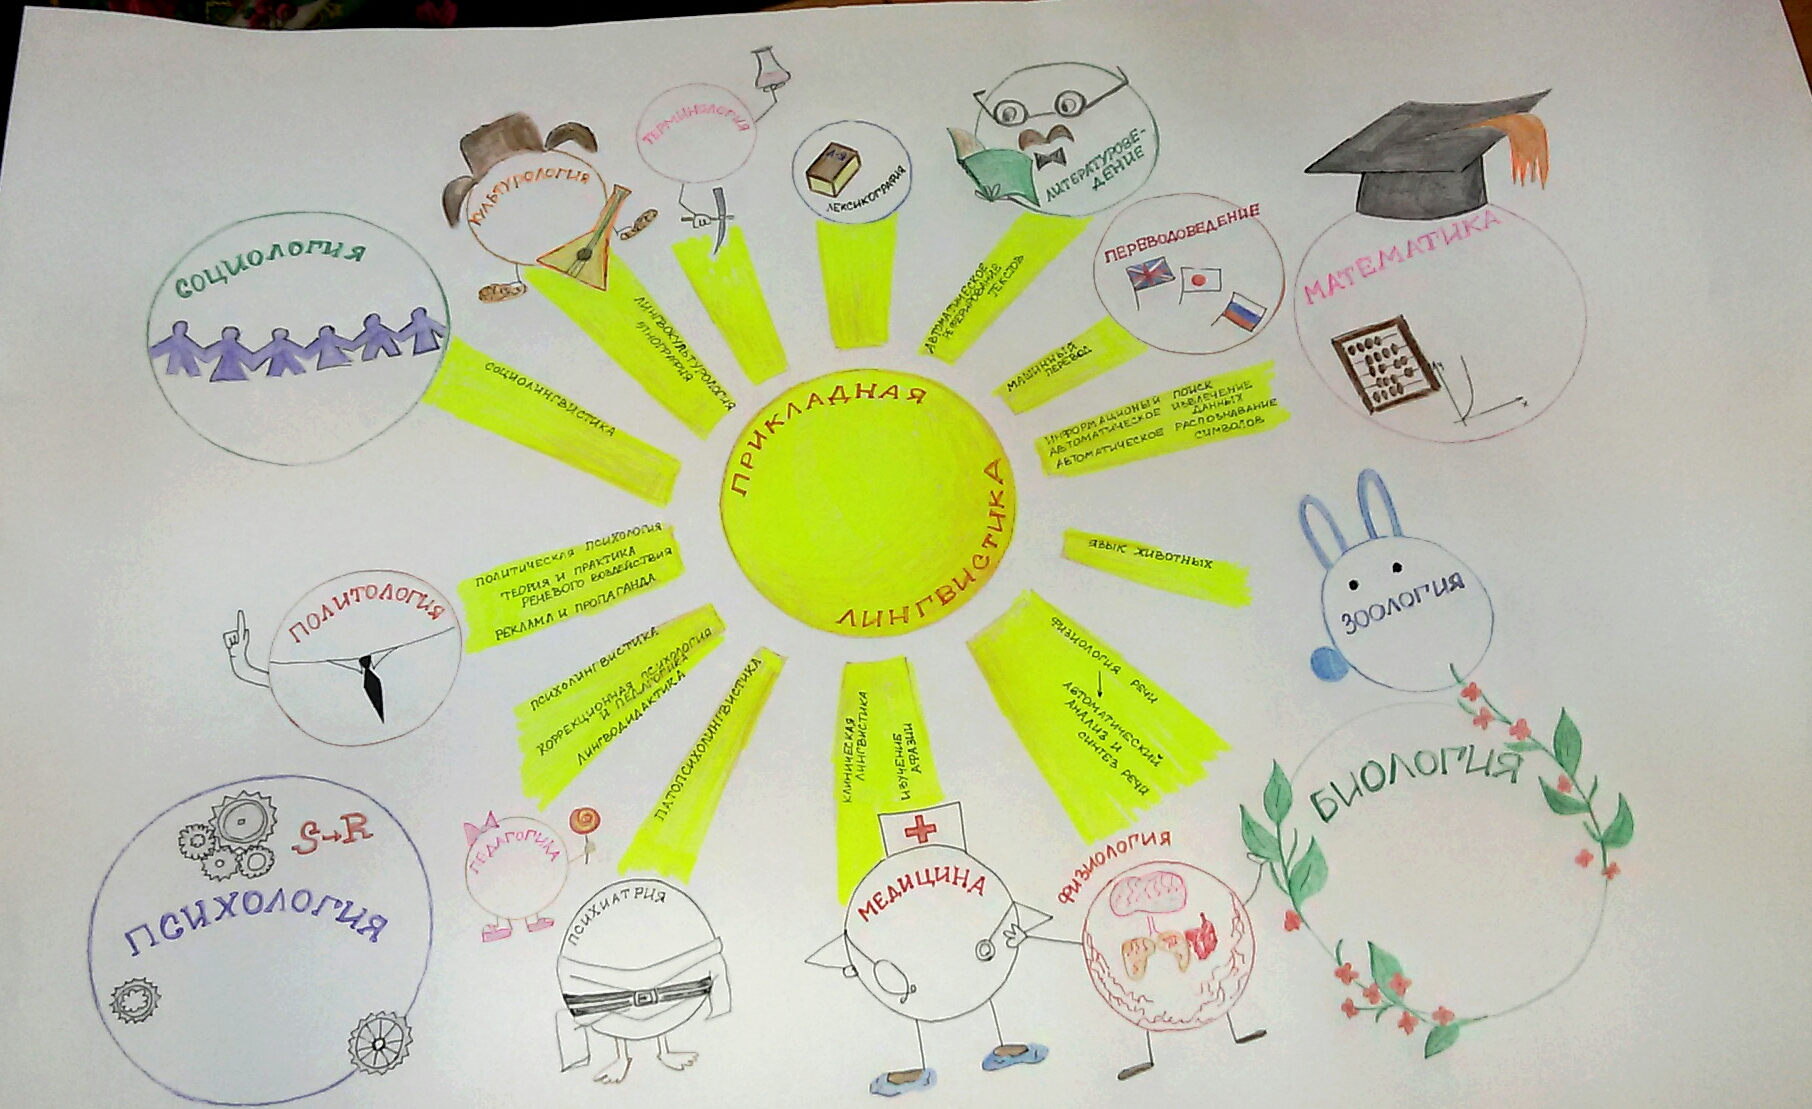
\includegraphics[width=.9\textwidth]{appl-ling}
\end{frame}

\begin{frame}{}
    \centering

    \vfill
    Q\&A
    \vfill
\end{frame}
